\documentclass[11pt,a4paper,landscape]{article}
\usepackage[utf8]{inputenc}
\usepackage[english]{babel}
\usepackage[left=2cm,right=2cm,top=2cm,bottom=2cm]{geometry}
\usepackage{fancyhdr}
\usepackage{multicol}
\usepackage{graphicx}
\usepackage{siunitx}
\usepackage{amsmath}
\usepackage{amssymb}
\usepackage{wrapfig}
\usepackage{float}
\usepackage{enumerate}

\author{Himanshu Mittal}
\title{Logs, surds and Indices}

\renewcommand{\labelenumi}{\theenumi}

\everymath{\displaystyle}
\pagestyle{fancy}
\fancyhf{}
\graphicspath{{./images/}}

\renewcommand{\headrulewidth}{0pt}
\renewcommand{\footrulewidth}{2pt}
\setlength\parindent{0pt}
\lfoot{\textbf{Himanshu Mittal : mittal01091997@gmail.com}}

\begin{document}
\begin{multicols*}{3}
\textbf{\Huge{Logs, Surds and Indices}}

\section{Indices}
	\begin{itemize}
	\item $a^2+b^2+c^2-ab-bc-ca$\\
	$=\frac{1}{2}\left[(a-b)^2+(b-c)^2+(c-a)^2\right]$
	\item $(a+b+c)^2=a^2+b^2+c^2+2(ab+bc+ca)$
	\item $(a+b)^3=a^3+b^3+3ab(a+b)$\\
		$(a-b)^3=a^3-b^3-3ab(a-b)$
	\item $a^3+b^3=(a+b)(a^2-ab+b^2)$\\
		$a^3-b^3=(a-b)(a^2+ab+b^2)$
	\item $a^3+b^3+c^3-3abc$\\
	$=(a+b+c)\left(a^2+b^2+c^2-ab-bc-ca\right)$\\
	$=\frac{1}{2}(a+b+c)\left((a-b)^2+(b-c)^2+(c-a)^2\right)$
	\item $a^n-b^n=(a-b)$\\
	$\left(a^{n-1}+a^{n-2}b+a^{n-3}b^2+\cdots+b^{n-1}\right)$\\
		$a^n+b^n=(a+b)$\\
		$\left(a^{n-1}-a^{n-2}b+a^{n-2}b^2-\cdots+ab^{n-2}-b^{n-1}\right)$
	\item If $\frac{a}{b}=\frac{c}{d}$ then,\\
		$\frac{a}{b}=\frac{c}{d}=\frac{a+c}{b+d}=\frac{\left(a^2+c^2\right)^{\frac{1}{2}}}{\left(b^2+d^2\right)^{\frac{1}{2}}}=\cdots$
	\end{itemize}
\vfill\null
\columnbreak
\section{Surds}
	\begin{itemize}
	\item $a+\sqrt{b}=c+\sqrt{d}\Leftrightarrow a=c\,\&\,b=d$
	\item $\sqrt{a+\sqrt{b}}=\sqrt{x}+\sqrt{y}\Leftrightarrow\sqrt{a-\sqrt{b}}=\sqrt{x}-\sqrt{y}$
	\item $\sqrt[3]{a+\sqrt{b}}=x+\sqrt{y}\Leftrightarrow\sqrt[3]{a-\sqrt{b}}=x-\sqrt{y}$
	\end{itemize}
\section{Logs}
	\begin{center}
	$b^p=n$\\
	$p=\log_b n$
	\end{center}
	\subsection{Cases:}
	\begin{itemize}
	\item If $n<0$, $\log_b n$ is imaginary
	\item If $n=0$, $\log_b n$ doesn't exist
	\item If $n>0$, $\log_b n$ exists for $b>0\,\&\,b \neq 1$
	\end{itemize}
	\subsection{Properties:}
	\begin{itemize}
	\item $b^{\log_b n}=n$
	\item $a^{\log_b n}=n^{\log_b a}$
	\item $\log_b b=1$, $\log_b 1=0$
	\item $\log_b n=\frac{1}{\log_n b}$
	\item $\log_b n=\log_a n\log_b a=\frac{\log_a n}{\log_a b}$
	\item $\log_b (mn)=\log_b m + \log_b n$
	\item $\log_b \left(\frac{m}{n}\right)=\log_b m - \log_b n$
	\item $\log_{b^a} n^x=\frac{x}{a}\log_b n$\\
		$\log_b n^x=x\log_b n$\\
		$\log_{b^a} n=\frac{1}{a}\log_b n$
	\item $\log_b n=\frac{\log n}{\log b}$
	\item $\log n=\log_e n$
	\item Common logarithms $\Rightarrow b=10$ (base 10)\\
		Natural logarithms $\Rightarrow b=e$ (base $e$)
	\end{itemize}
	\subsection{Useful Results}
	\textbf{Result 1} If $b>1$, then
	\begin{figure}[H]
		\centering
		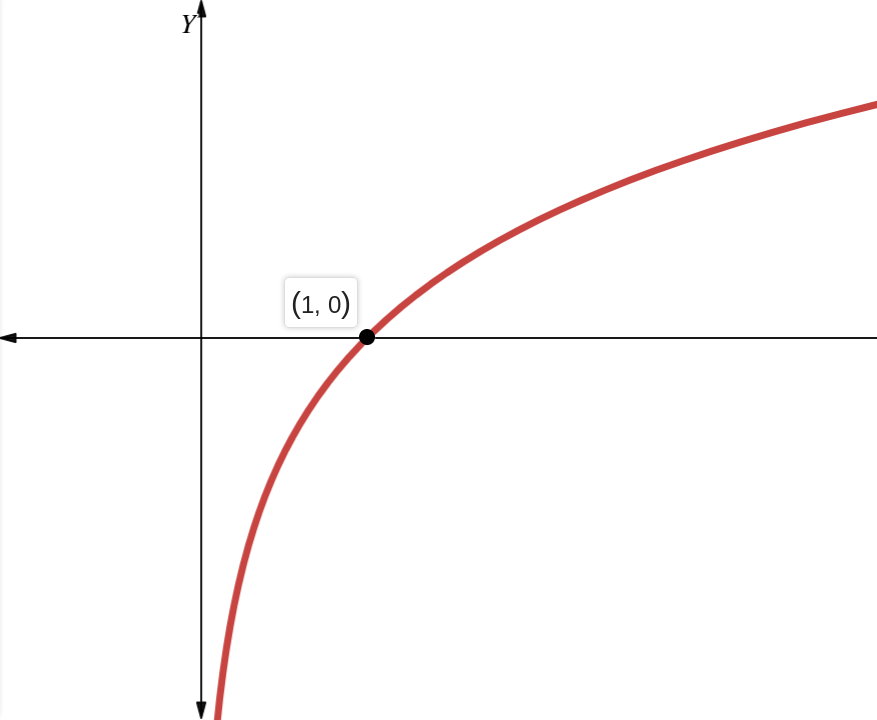
\includegraphics[width=6cm]{final2.png}
		\caption{Graph for $y=\log_b n , b>1$}
	\end{figure}
	\begin{itemize}
		\item $\log_b n < 0 \Rightarrow 0<n<1$
		\item $\log_b n =0 \Rightarrow n=1$
		\item $\log_b n >0 \Rightarrow n>1$
		\item $x>y \Rightarrow \log_b x > \log_b y$
		\item $\log_b n$ is an increasing function.
		\item $n>b \Rightarrow \log_b n >1$
		\item $0<n<b \Rightarrow \log_b n <1$
		\item $n=b \Rightarrow \log_b n =1$
	\end{itemize}
	\textbf{Result 2} If $0<b<1$, then
	\begin{figure}[H]
		\centering
		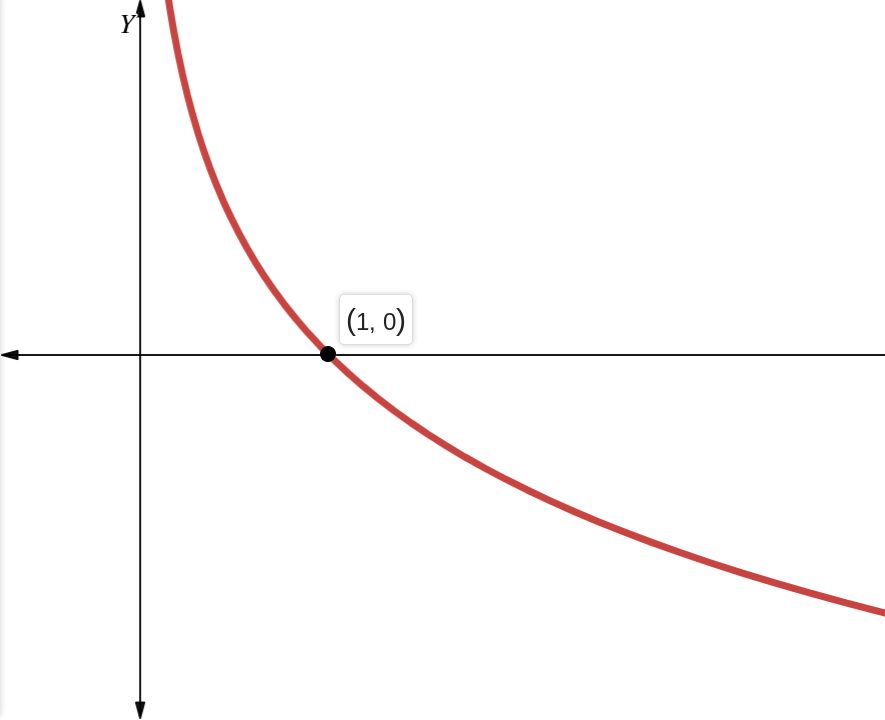
\includegraphics[width=6cm]{final1.png}
		\caption{Graph for $y=\log_b n , 0<b<1$}
	\end{figure}
	\begin{itemize}
		\item $\log_b n <0 \Rightarrow n>1$
		\item $\log_b n =0 \Rightarrow n=1$
		\item $\log_b n >0 \Rightarrow 0<n<1$
		\item $x>y \Rightarrow \log_b x < \log_b y$
		\item $\log_b n$ is an decreasing function.
		\item $0<n<b \Rightarrow \log_b n >1$
		\item $n=b \Rightarrow \log_b n =1$
		\item $n>b \Rightarrow \log_b n <1$
	\end{itemize}
\section{Componento and Dividendo}
	If $\frac{p}{q}=\frac{a}{b}$, then:
	\begin{description}
	\item $\frac{p-q}{p+q}=\frac{a-b}{a+b}$ or, $\frac{p+q}{p-q}=\frac{a+b}{a-b}$
	\item $\frac{q-p}{q+p}=\frac{b-a}{b+a}$ or, $\frac{q+p}{q-p}=\frac{b+a}{b-a}$
	\end{description}
\section{Rule of Cross Multiplication}
	Consider Equations:\\
	$a_1x+b_1y+c_1z=0$ and $a_2x+b_2y+c_2z=0$\\
	\begin{figure}[H]
		\centering
		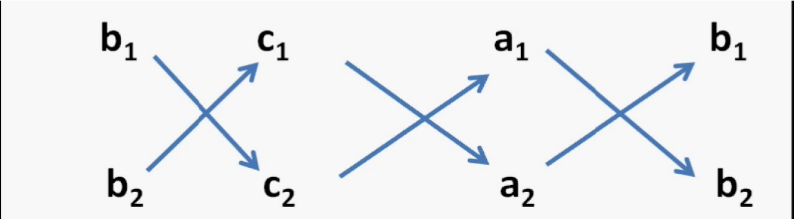
\includegraphics[width=8cm]{maxresdefault2.png}
		\caption{Cross Products for $x,y\,and\,z$}
	\end{figure}
	\begin{center}
	$\frac{x}{b_1c_2-c_1b_2}=\frac{y}{c_1a_2-a_1c_2}=\frac{z}{a_1b_2-b_1a_2}$ 
	\end{center}
	\vfill\null
\end{multicols*}
\end{document}
